$  $% !TeX spellcheck = de_DE
%Die Angabe des schlauen Spruchs auf diesem Wege funtioniert nur,
%wenn keine Änderung des Kapitels mittels den in preambel/chapterheads.tex
%vorgeschlagenen Möglichkeiten durchgeführt wurde.
\setchapterpreamble[u]{%
	\dictum[Albert Einstein]{Probleme kann man niemals mit derselben Denkweise lösen, durch die sie entstanden sind.}
}
\chapter{Additional OBSW examples}
\label{chap: Extra examples}

The code generator implemented as a part of this Master thesis, is also tested for other example OBSW models, designed using the OSRA SCM Model editor. Each of these examples are carefully constructed to capture all the corner cases listed in the section \cref{section: Corner cases}. The complexity of each of these models is much higher when compared to the simple OSRA example model introduced in \cref{chap: Code generation}.

\section{Producer/Consumer problem}
This problem is one of the problems in the collection of standard, well-known problems in concurrent programming domain. In this classical problem \cite{ProducerConsumer}, there are two entities specifically producers and consumers. Producers put items into the buffer and the consumers take items out of the buffer. Additionally a producer must wait until the buffer has space before it can put something in, and a consumer must wait until something is in buffer before it can take something out. In this example, we have two producers and one consumer. The figures in the \cref{fig: FiguresPC} and the tables \cref{table: RIPortsPC}, \cref{table: PIPortsPC} and \cref{table: EventsPC} give an idea about how this example is constructed.   

\begin{figure}[h]
	\centering
	\subfloat[Data types, events, exceptions and interfaces diagram]{%
		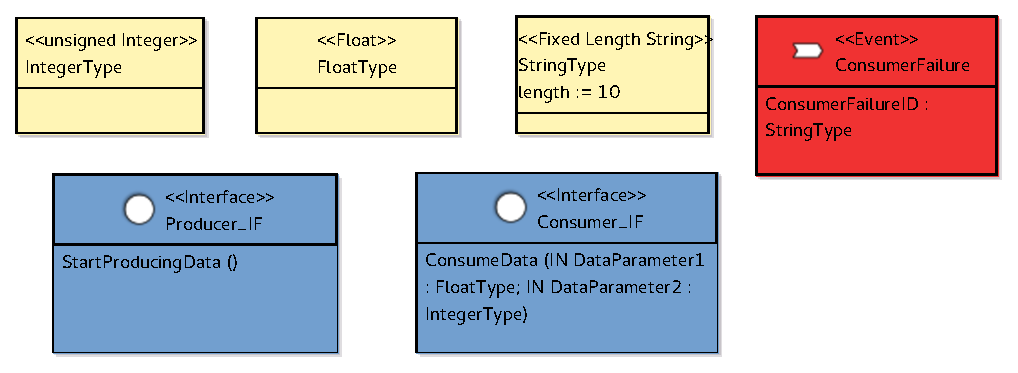
\includegraphics[width=0.8\columnwidth,keepaspectratio]{InterfacesEventsDatasetsDiagramPC.pdf}
	}\hfill
	\subfloat[Component types diagram]{%
		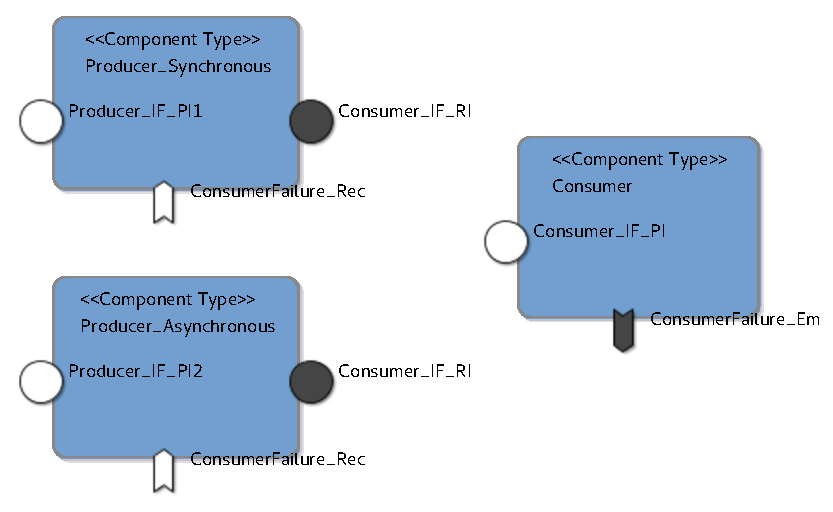
\includegraphics[width=0.8\columnwidth,keepaspectratio]{ComponentTypesDiagramPC.pdf}
	}\hfill
	\subfloat[Component instances diagram]{%
		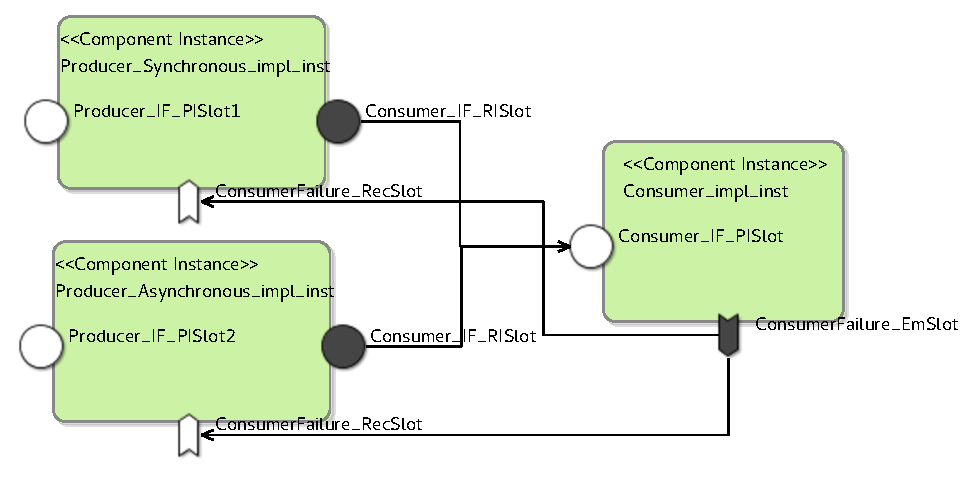
\includegraphics[width=0.8\columnwidth,keepaspectratio]{ComponentInstancesDiagramPC.pdf}
	}%
	\label{fig: FiguresPC}
	\caption{Producer/Consumer example}
\end{figure}

\begin{table}[h]
	\centering
	\caption{Desired interaction kind for operations in the required interface ports}
	\label{table: RIPortsPC}
	\begin{tabular}{|c|c|c|c|}
		\hline
		\textbf{Component type} & \textbf{Required interface ports} & \textbf{Operations} & \textbf{Interaction kind} \\ \hline
		Producer\_Synchronous & Consumer\_IF\_RI & ConsumeData & synchronous \\ \hline
		Producer\_Asynchronous & Consumer\_IF\_RI & ConsumeData & asynchronous \\ \hline
	\end{tabular}
\end{table}

\begin{table}[h]
	\centering
	\caption{Non-functional properties for the operations in the provided interface slots}
	\label{table: PIPortsPC}
	\begin{tabular}{|c|c|c|}
		\hline
		\textbf{Provided interface slot} & \textbf{Operation} & \textbf{Non-functional property} \\ \hline
		Producer\_IF\_PISlot1 & StartProducingData & Cyclic, Period = 2s \\ \hline
		Producer\_IF\_PISlot2 & StartProducingData & Cyclic, Period = 3s \\ \hline
		Consumer\_IF\_PISlot & ConsumeData & Protected \\ \hline
	\end{tabular}
\end{table}

% Please add the following required packages to your document preamble:
% \usepackage{graphicx}
\begin{table}[h]
	\centering
	\caption{Non-functional property for event reception}
	\label{table: EventsPC}
	\resizebox{\textwidth}{!}{%
		\begin{tabular}{|c|c|c|c|}
			\hline
			\textbf{Component type} & \textbf{Event receiver slot} & \textbf{Event} & \textbf{Non-functional property} \\ \hline
			Producer\_Synchronous & ConsumerFailure\_RecSlot & ConsumerFailure & Protected \\ \hline
			Producer\_Asynchronous & ConsumerFailure\_RecSlot & ConsumerFailure & Unprotected \\ \hline
		\end{tabular}%
	}
\end{table}


\section{Building block approach}
The Component based approach is one of the high level requirements discussed in the \cref{chap:OSRA}. According to this requirement, it should be possible to design the software as a combination of reusable units. The reusable units, being component instances, the aim of this example to reiterate the CBSE approach by having multiple component instances which correspond to the same component type. The figures in the \cref{fig: FiguresBB} and the tables \cref{table: RIPortsBB} and \cref{table: PIPortsBB} give an idea about how this example is constructed.

\begin{figure}[h]
	\centering
	\subfloat[Data types, events, exceptions and interfaces diagram]{%
		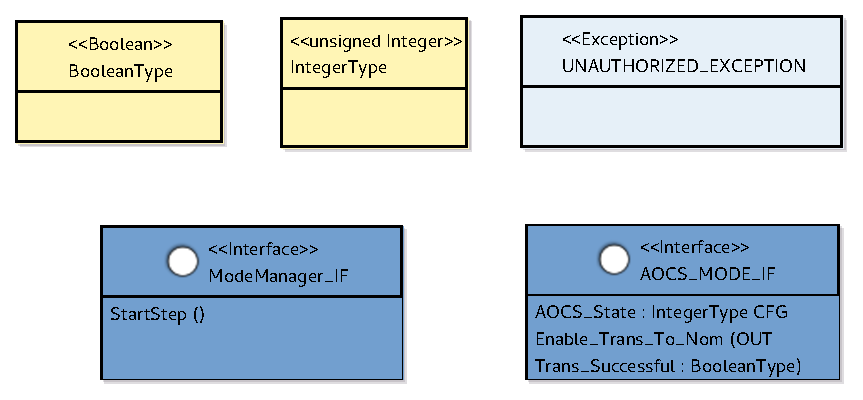
\includegraphics[width=0.8\columnwidth,keepaspectratio]{InterfacesEventsDatasetsDiagramBBA.pdf}
	}\hfill
	\subfloat[Component types diagram]{%
		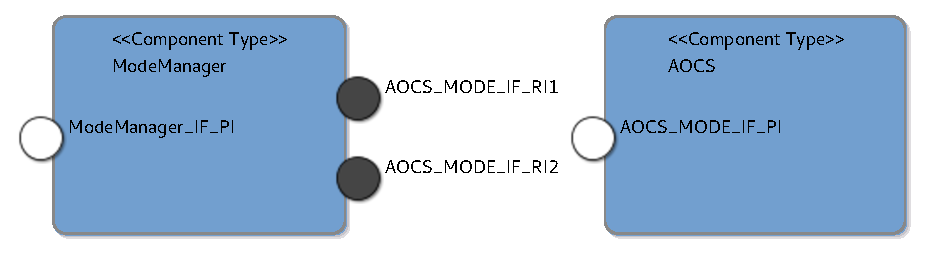
\includegraphics[width=0.8\columnwidth,keepaspectratio]{ComponentTypesDiagramBBA.pdf}
	}\hfill
	\subfloat[Component instances diagram]{%
		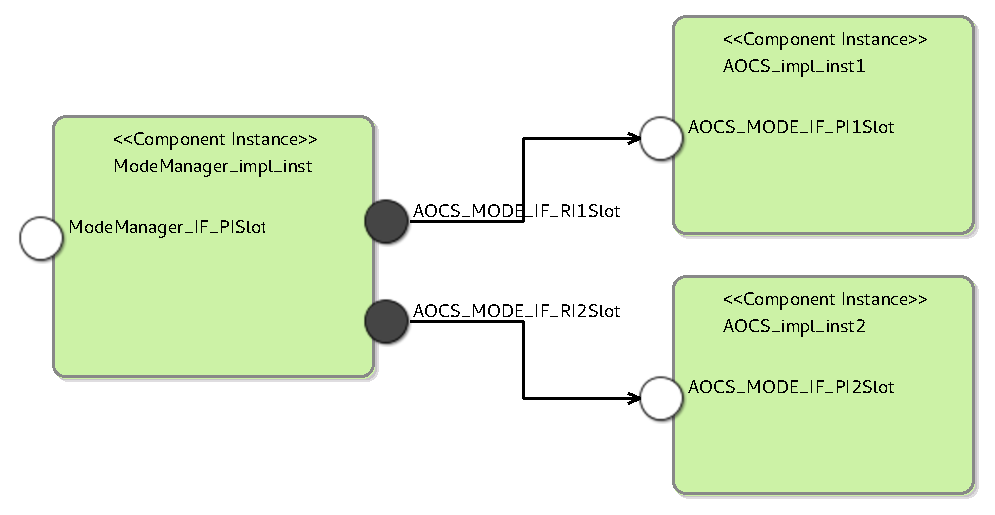
\includegraphics[width=0.8\columnwidth,keepaspectratio]{ComponentInstancesDiagramBBA.pdf}
	}%
	\label {fig: FiguresBB}
	\caption{Building block approach example}
\end{figure}

\begin{table}[h]
	\centering
	\caption{Desired interaction kind for operations in the required interface ports}
	\label{table: RIPortsBB}
	\begin{tabular}{|c|c|c|}
		\hline
		\textbf{Required interface ports} & \textbf{Operations} & \textbf{Interaction kind} \\ \hline
		AOCS\_MODE\_IF\_RI1 & \begin{tabular}[c]{@{}c@{}}Enable\_Trans\_To\_Nom\\ AOCS\_State setter\\ AOCS\_State getter\end{tabular} & \begin{tabular}[c]{@{}c@{}}asynchronous\\ synchronous\\ asynchronous\end{tabular} \\ \hline
		AOCS\_MODE\_IF\_RI2 & \begin{tabular}[c]{@{}c@{}}Enable\_Trans\_To\_Nom\\ AOCS\_State setter\\ AOCS\_State getter\end{tabular} & \begin{tabular}[c]{@{}c@{}}synchronous\\ asynchronous\\ synchronous\end{tabular} \\ \hline
	\end{tabular}
\end{table}

\begin{table}[h]
	\centering
	\caption{Non-functional properties for the operations in the provided interface slots}
	\label{table: PIPortsBB}
	\begin{tabular}{|c|c|c|}
		\hline
		\textbf{Provided interface slot} & \textbf{Operation} & \textbf{Non-functional property} \\ \hline
		Mode\_Manager\_IF\_PISlot & StartStep & Cyclic, Period = 4s \\ \hline
		AOCS\_MODE\_IF\_PI1Slot & \begin{tabular}[c]{@{}c@{}}Enable\_Trans\_To\_Nom\\ AOCS\_State getter\\ AOCS\_State setter\end{tabular} & \begin{tabular}[c]{@{}c@{}}Sporadic, MIAT = 2s\\ Protected\\ Protected\end{tabular} \\ \hline
		AOCS\_MODE\_IF\_PI2Slot & \begin{tabular}[c]{@{}c@{}}Enable\_Trans\_To\_Nom\\ AOCS\_State getter\\ AOCS\_State setter\end{tabular} & \begin{tabular}[c]{@{}c@{}}Protected\\ Protected\\ Protected\end{tabular} \\ \hline
	\end{tabular}
\end{table}

\section{Component chaining}
As discussed before in the initial chapters, the composability and compositionality are one the corner-stone principles of the OSRA. In line with these corner-stone principles, this example aims to chain different types of components together. The figures in the \cref{fig: FiguresCC} and the tables \cref{table: RIPortsCC}, \cref{table: PIPortsCC} and \cref{table: EventsCC} give an idea about how this example is constructed.

\begin{figure}[h]
	\centering
	\subfloat[Data types, events, exceptions and interfaces diagram]{%
		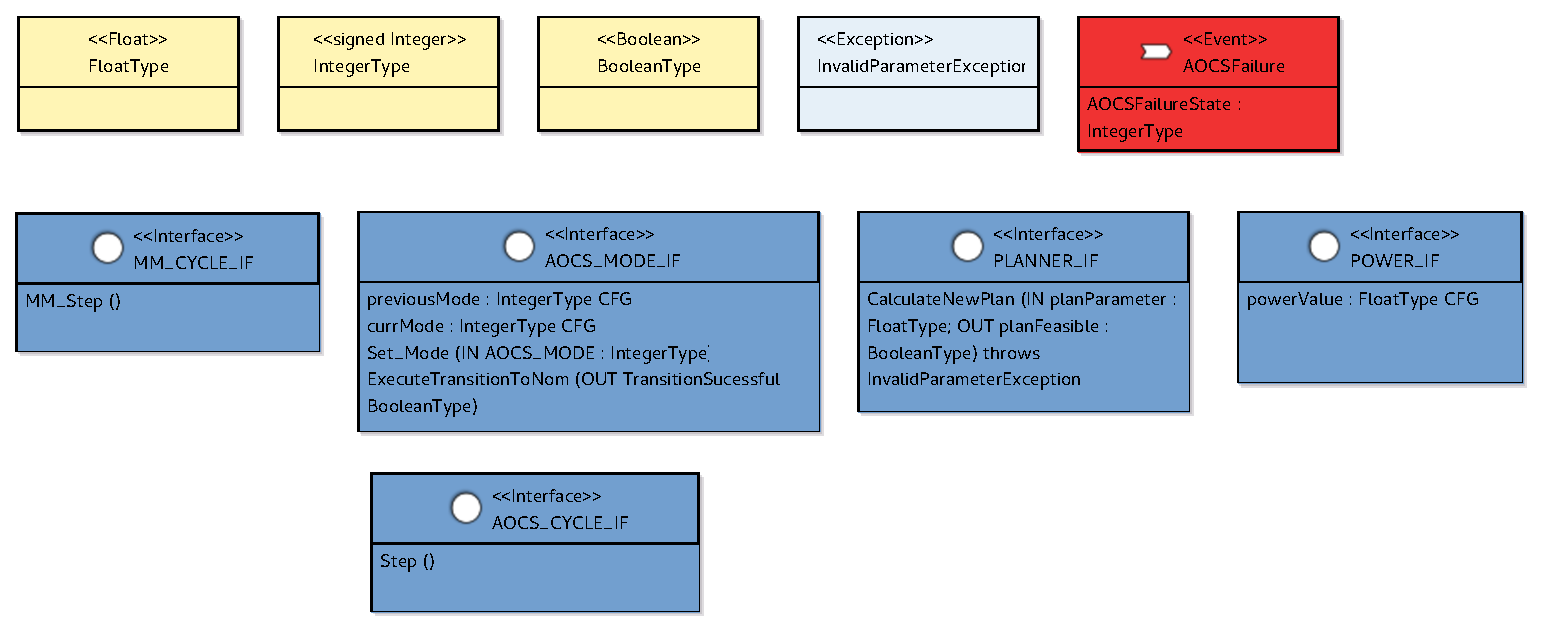
\includegraphics[width=1.0\columnwidth,keepaspectratio]{InterfacesEventsDatasetsDiagramCC.pdf}
	}\hfill
	\subfloat[Component types diagram]{%
		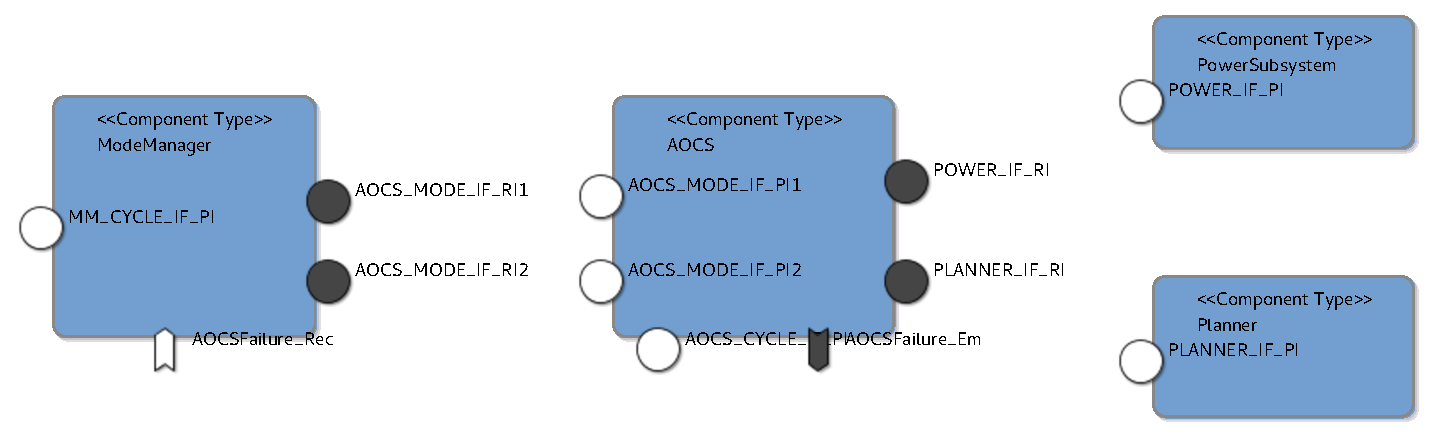
\includegraphics[width=1.0\columnwidth,keepaspectratio]{ComponentTypesDiagramCC.pdf}
	}\hfill
	\subfloat[Component instances diagram]{%
		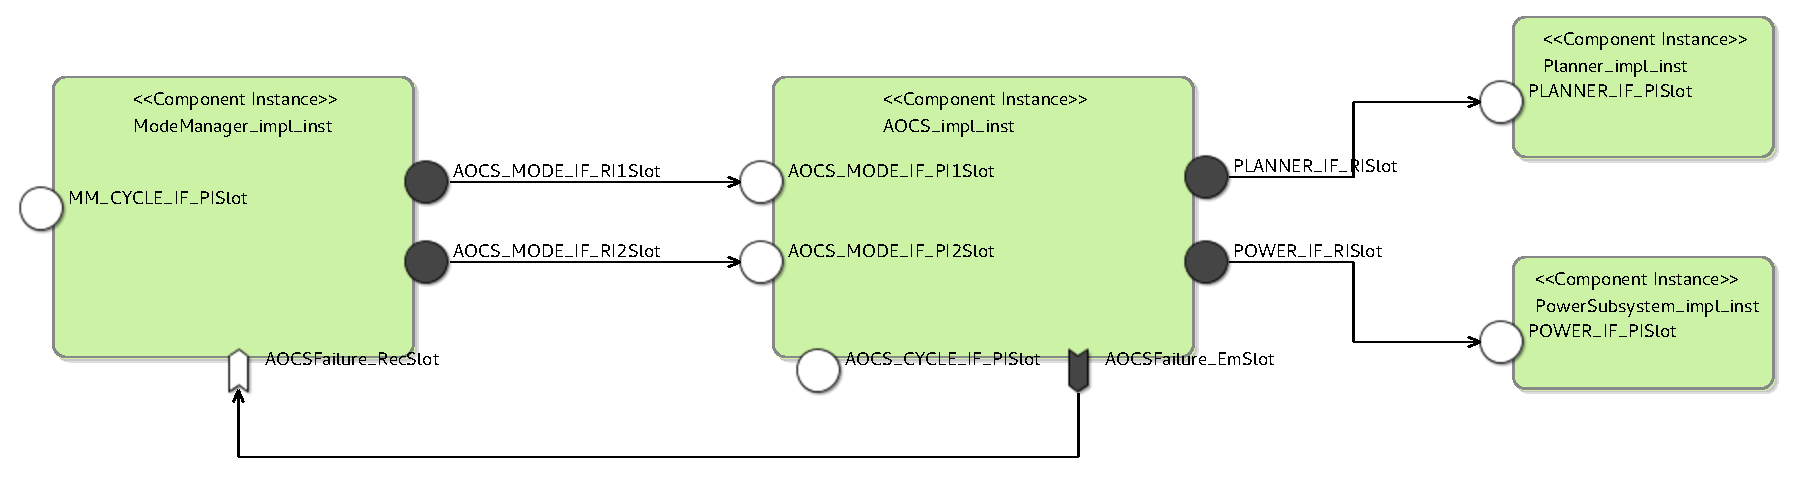
\includegraphics[width=1.0\columnwidth,keepaspectratio]{ComponentInstancesDiagramCC.pdf}
	}%
	\label{fig: FiguresCC}
	\caption{Component chaining example}
\end{figure}

\begin{table}[h]
	\centering
	\caption{Desired interaction kind for operations in the required interface ports}
	\label{table: RIPortsCC}
	\begin{tabular}{|c|c|c|}
		\hline
		\textbf{Required interface ports} & \textbf{Operations} & \textbf{Interaction kind} \\ \hline
		AOCS\_MODE\_IF\_RI1 & \begin{tabular}[c]{@{}c@{}}Set\_Mode\\ ExecuteTransitionToNom\\ previousMode getter\\ previousMode setter\\ currMode getter\\ currMode setter\end{tabular} & \begin{tabular}[c]{@{}c@{}}asynchronous\\ synchronous\\ asynchronous\\ synchronous\\ synchronous\\ asynchronous\end{tabular} \\ \hline
		AOCS\_MODE\_IF\_RI2 & \begin{tabular}[c]{@{}c@{}}Set\_Mode\\ ExecuteTransitionToNom\\ previousMode getter\\ previousMode setter\\ currMode getter\\ currMode setter\end{tabular} & \begin{tabular}[c]{@{}c@{}}asynchronous\\ asynchronous\\ synchronous\\ asynchronous\\ asynchronous\\ synchronous\end{tabular} \\ \hline
		POWER\_IF\_RI & \begin{tabular}[c]{@{}c@{}}powerValue getter\\ powerValue setter\end{tabular} & \begin{tabular}[c]{@{}c@{}}asynchronous\\ asynchronous\end{tabular} \\ \hline
		PLANNER\_IF\_RI & calculateNewPlan & synchronous \\ \hline
	\end{tabular}
\end{table}

\begin{table}[h]
	\centering
	\caption{Non-functional properties for the operations in the provided interface slots}
	\label{table: PIPortsCC}
	\begin{tabular}{|c|c|c|}
		\hline
		\textbf{Provided interface slot} & \textbf{Operation} & \textbf{Non-functional property} \\ \hline
		MM\_CYCLE\_IF\_PISlot & MM\_Step & Cyclic, Period = 2s \\ \hline
		AOCS\_MODE\_IF\_PI1Slot & \begin{tabular}[c]{@{}c@{}}Set\_Mode\\ ExecuteTransitionToNom\\ previousMode getter\\ previousMode setter\\ currMode getter\\ currMode setter\end{tabular} & \begin{tabular}[c]{@{}c@{}}Sporadic, MIAT = 3s\\ Unprotected\\ Protected \\ Protected\\ Protected\\ Protected\end{tabular} \\ \hline
		AOCS\_MODE\_IF\_PI2Slot & \begin{tabular}[c]{@{}c@{}}Set\_Mode\\ ExecuteTransitionToNom\\ previousMode getter\\ previousMode setter\\ currMode getter\\ currMode setter\end{tabular} & \begin{tabular}[c]{@{}c@{}}Protected\\ Protected\\ Protected\\ Protected\\ Protected\\ Protected\end{tabular} \\ \hline
		AOCS\_CYCLE\_IFPIslot & Step & Cyclic, Period = 4s \\ \hline
		PLANNER\_IF\_PISlot & CalculateNewPlan & Unprotected \\ \hline
		POWER\_IF\_PISlot & \begin{tabular}[c]{@{}c@{}}powerValue getter\\ powerValue setter\end{tabular} & \begin{tabular}[c]{@{}c@{}}Protected\\ Protected\end{tabular} \\ \hline
	\end{tabular}
\end{table}

\begin{table}[H]
	\centering
	\caption{Non-functional property for event reception}
	\label{table: EventsCC}
	\begin{tabular}{|c|c|c|}
		\hline
		\textbf{Event receiver slot} & \textbf{Event} & \textbf{Non-functional property} \\ \hline
		AOCSFailure\_RecSlot & AOCSFailure & Unprotected \\ \hline
	\end{tabular}
\end{table}

\section{Cyclic dependency}
This example takes into consideration the situation wherein the components are dependent on each other in such a way that there is a cyclic dependency. The expectation that this cyclic dependency should still be handled by the code generator efficiently is tested in this example. The figures in the \cref{fig: FiguresCD} and the tables \cref{table: RIPortsCD}, \cref{table: PIPortsCD} and \cref{table: EventsCD} give an idea about how this example is constructed.

\begin{figure}[h]
	\centering
	\subfloat[Data types, events, exceptions and interfaces diagram]{%
		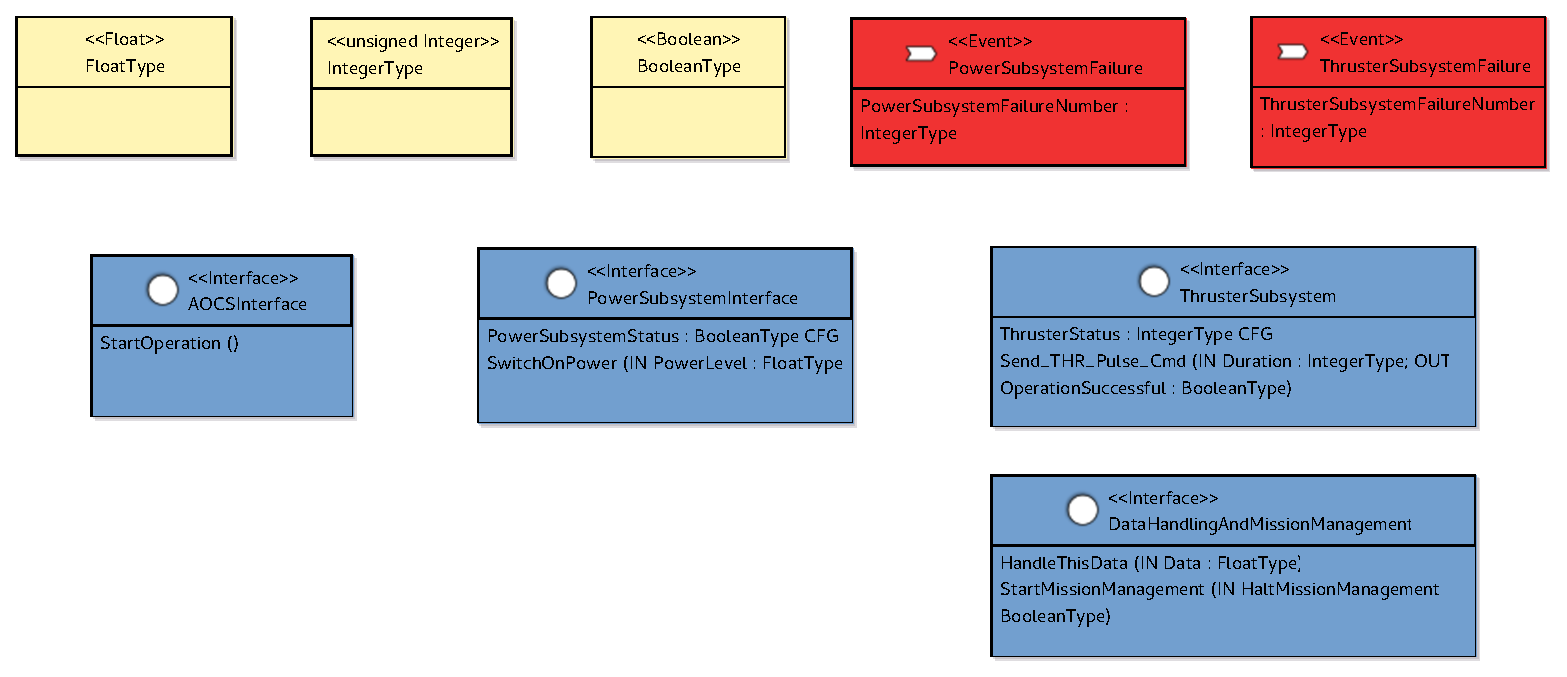
\includegraphics[width=1.0\columnwidth,keepaspectratio]{InterfacesEventsDatasetsDiagramCD.pdf}
	}\hfill
	\subfloat[Component types diagram]{%
		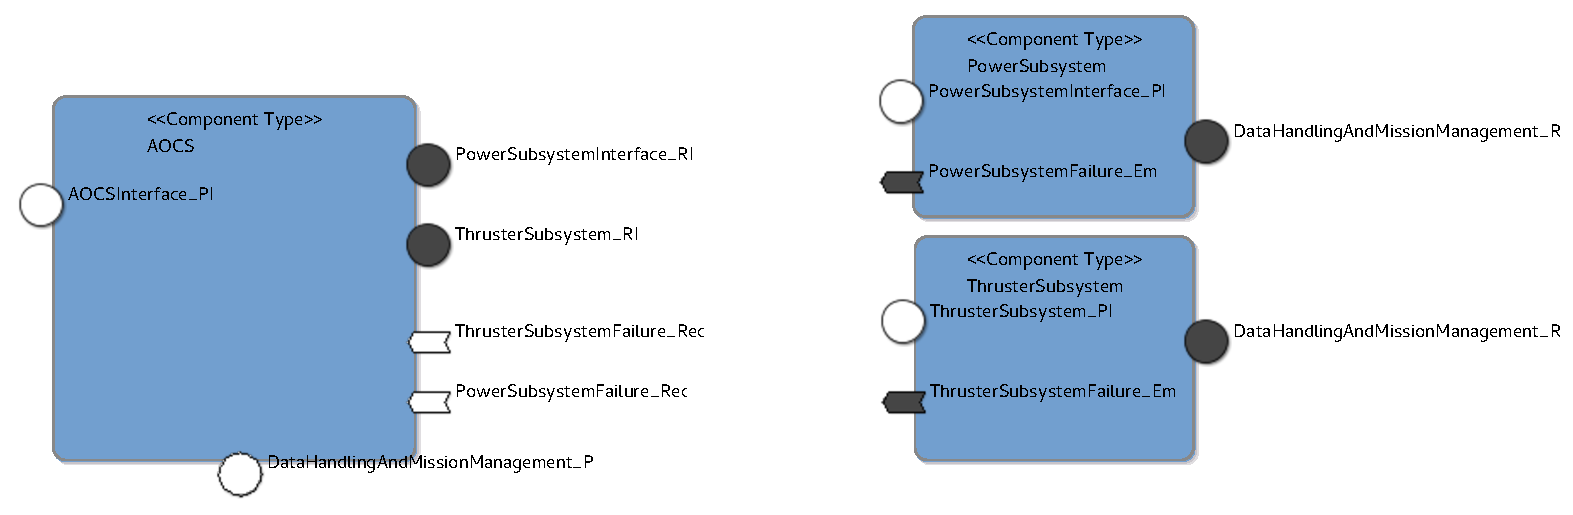
\includegraphics[width=1.0\columnwidth,keepaspectratio]{ComponentTypesDiagramCD.pdf}
	}\hfill
	\subfloat[Component instances diagram]{%
		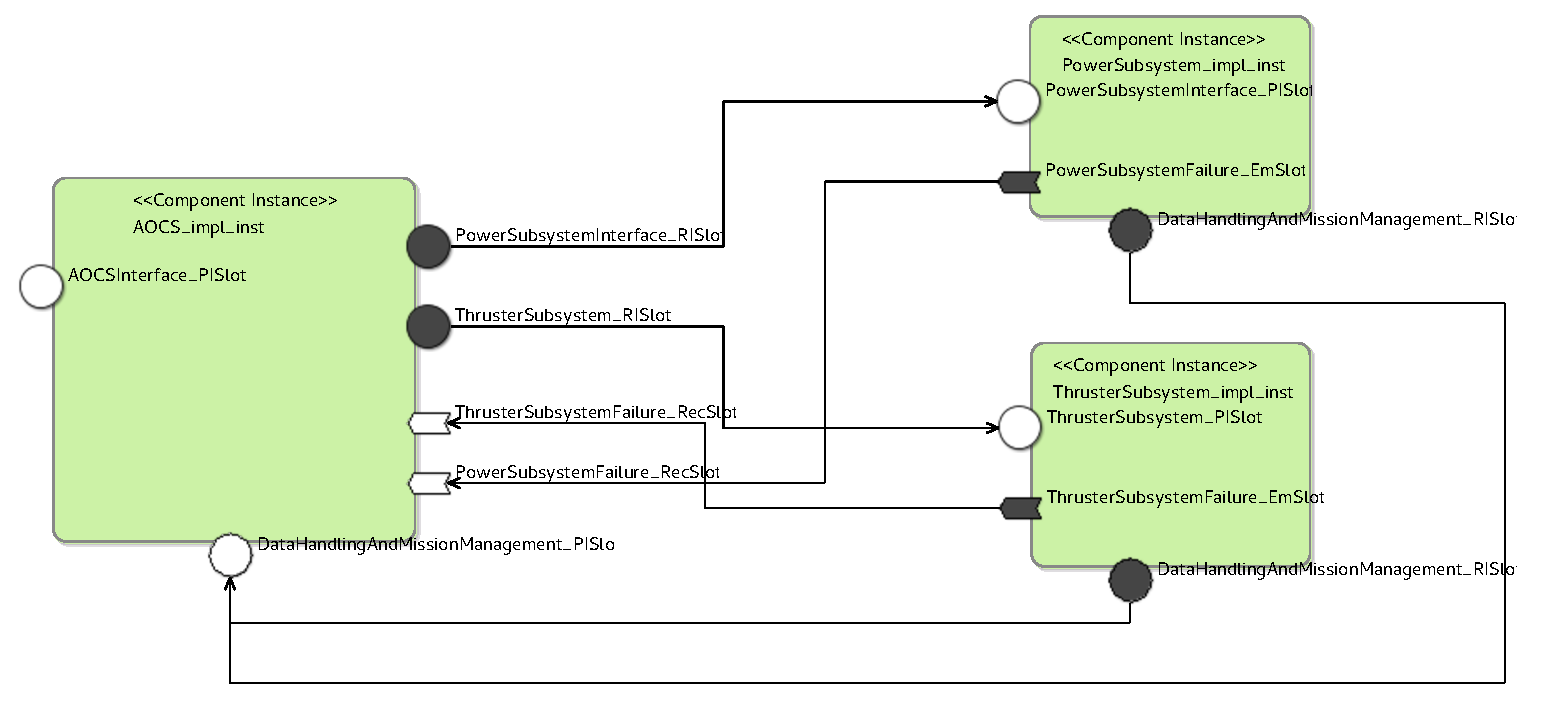
\includegraphics[width=1.0\columnwidth,keepaspectratio]{ComponentInstancesDiagramCD.pdf}
	}%
	\label{fig: FiguresCD}
	\caption{Cyclic dependency example}
\end{figure}

% Please add the following required packages to your document preamble:
% \usepackage{graphicx}
\begin{table}[h]
	\centering
	\caption{Desired interaction kind for operations in the required interface ports}
	\label{table: RIPortsCD}
	\resizebox{\textwidth}{!}{%
		\begin{tabular}{|c|c|c|c|}
			\hline
			\textbf{Component type} & \textbf{Required interface ports} & \textbf{Operations} & \textbf{Interaction kind} \\ \hline
			AOCS & PowerSubsystemInterface\_RI & \begin{tabular}[c]{@{}c@{}}SwitchOnPower\\ PowerSubsystemStatus getter\\ PowerSubsystemStatus setter\end{tabular} & \begin{tabular}[c]{@{}c@{}}asynchronous\\ synchronous\\ synchronous\end{tabular} \\ \hline
			AOCS & ThrusterSubsystem\_RI & \begin{tabular}[c]{@{}c@{}}Send\_THR\_Pulse\_CMD\\ ThrusterStatus getter\\ ThrusterStatus setter\end{tabular} & \begin{tabular}[c]{@{}c@{}}synchronous\\ asynchronous\\ asynchronous\end{tabular} \\ \hline
			PowerSubsystem & DataHandlingAndMissionManagement\_RI & \begin{tabular}[c]{@{}c@{}}HandleThisData\\ StartMissionManagement\end{tabular} & \begin{tabular}[c]{@{}c@{}}asynchronous\\ synchronous\end{tabular} \\ \hline
			ThrusterSubsystem & DataHandlingAndMissionManagement\_RI & \begin{tabular}[c]{@{}c@{}}HandleThisData\\ StartMissionManagement\end{tabular} & \begin{tabular}[c]{@{}c@{}}synchronous\\ asynchronous\end{tabular} \\ \hline
		\end{tabular}%
	}
\end{table}

% Please add the following required packages to your document preamble:
% \usepackage{graphicx}
\begin{table}[h]
	\centering
	\caption{Non-functional properties for the operations in the provided interface slots}
	\label{table: PIPortsCD}
	\resizebox{\textwidth}{!}{%
		\begin{tabular}{|c|c|c|}
			\hline
			\textbf{Provided interface slot} & \textbf{Operation} & \textbf{Non-functional property} \\ \hline
			AOCSInterface\_PISlot & StartOperation & Cyclic, Period = 2s \\ \hline
			DataHandlingAndMissionManagement\_PISlot & \begin{tabular}[c]{@{}c@{}}HandleThisData\\ StartMissionManagement\end{tabular} & \begin{tabular}[c]{@{}c@{}}Protected\\ Protected\end{tabular} \\ \hline
			PowerSubsystemInterface\_PISlot & \begin{tabular}[c]{@{}c@{}}SwitchOnPower\\ PowerSubsystemStatus getter\\ PowerSubsystemStatus setter\end{tabular} & \begin{tabular}[c]{@{}c@{}}Sporadic, MIAT = 2s\\ Protected\\ Protected\end{tabular} \\ \hline
			ThrusterSubsystem\_PISlot & \begin{tabular}[c]{@{}c@{}}Send\_THR\_Pulse\_Cmd\\ ThrusterStatus getter\\ ThrusterStatus setter\end{tabular} & \begin{tabular}[c]{@{}c@{}}Unprotected\\ Protected\\ Protected\end{tabular} \\ \hline
		\end{tabular}%
	}
\end{table}

% Please add the following required packages to your document preamble:
% \usepackage{graphicx}
\begin{table}[h]
	\centering
	\caption{Non-functional property for event reception}
	\label{table: EventsCD}
	\resizebox{\textwidth}{!}{%
		\begin{tabular}{|c|c|c|}
			\hline
			\textbf{Event receiver slot} & \textbf{Event} & \textbf{Non-functional property} \\ \hline
			ThrusterSubsystemFailure\_RecSlot & ThrusterSubsystemFailure & Protected \\ \hline
			PowerSubsystemFailure\_RecSlot & PowerSubsystemFailure & Protected \\ \hline
		\end{tabular}%
	}
\end{table}



 




   
 